\documentclass[12pt,a4paper,]{article}
\usepackage{lmodern}
\usepackage{amssymb,amsmath}
\usepackage{ifxetex,ifluatex}
\usepackage{fixltx2e} % provides \textsubscript
\ifnum 0\ifxetex 1\fi\ifluatex 1\fi=0 % if pdftex
  \usepackage[T1]{fontenc}
  \usepackage[utf8]{inputenc}
\else % if luatex or xelatex
  \ifxetex
    \usepackage{mathspec}
  \else
    \usepackage{fontspec}
  \fi
  \defaultfontfeatures{Ligatures=TeX,Scale=MatchLowercase}
    \setmainfont[]{Lato}
\fi
% use upquote if available, for straight quotes in verbatim environments
\IfFileExists{upquote.sty}{\usepackage{upquote}}{}
% use microtype if available
\IfFileExists{microtype.sty}{%
\usepackage{microtype}
\UseMicrotypeSet[protrusion]{basicmath} % disable protrusion for tt fonts
}{}
\usepackage[margin=1in]{geometry}
\usepackage{hyperref}
\hypersetup{unicode=true,
            pdftitle={A new method for modelling electroglottographic data},
            pdfauthor={Stefano Coretta},
            pdfborder={0 0 0},
            breaklinks=true}
\urlstyle{same}  % don't use monospace font for urls
\usepackage{natbib}
\bibliographystyle{unified}
\usepackage{graphicx,grffile}
\makeatletter
\def\maxwidth{\ifdim\Gin@nat@width>\linewidth\linewidth\else\Gin@nat@width\fi}
\def\maxheight{\ifdim\Gin@nat@height>\textheight\textheight\else\Gin@nat@height\fi}
\makeatother
% Scale images if necessary, so that they will not overflow the page
% margins by default, and it is still possible to overwrite the defaults
% using explicit options in \includegraphics[width, height, ...]{}
\setkeys{Gin}{width=\maxwidth,height=\maxheight,keepaspectratio}
\setlength{\emergencystretch}{3em}  % prevent overfull lines
\providecommand{\tightlist}{%
  \setlength{\itemsep}{0pt}\setlength{\parskip}{0pt}}
\setcounter{secnumdepth}{5}
% Redefines (sub)paragraphs to behave more like sections
\ifx\paragraph\undefined\else
\let\oldparagraph\paragraph
\renewcommand{\paragraph}[1]{\oldparagraph{#1}\mbox{}}
\fi
\ifx\subparagraph\undefined\else
\let\oldsubparagraph\subparagraph
\renewcommand{\subparagraph}[1]{\oldsubparagraph{#1}\mbox{}}
\fi

%%% Use protect on footnotes to avoid problems with footnotes in titles
\let\rmarkdownfootnote\footnote%
\def\footnote{\protect\rmarkdownfootnote}

%%% Change title format to be more compact
\usepackage{titling}

% Create subtitle command for use in maketitle
\providecommand{\subtitle}[1]{
  \posttitle{
    \begin{center}\large#1\end{center}
    }
}

\setlength{\droptitle}{-2em}

  \title{A new method for modelling electroglottographic data}
    \pretitle{\vspace{\droptitle}\centering\huge}
  \posttitle{\par}
    \author{Stefano Coretta}
    \preauthor{\centering\large\emph}
  \postauthor{\par}
    \date{}
    \predate{}\postdate{}
  
\usepackage{cleveref}

\begin{document}
\maketitle

\hypertarget{electroglottography}{%
\section{Electroglottography}\label{electroglottography}}

The position of the vocal folds within the oral tract makes
investigation about them difficult. Direct observation of the activity
of the larynx via invasive methods, like laryngoscopy and \ldots{},
brings with it a series of practical drawback. Among other methods for
obtaining information about glottal activity is electroglottography
{[}\ldots{}{]}. Electroglottography, or EGG, \citep{fabre1957} is a
technique that measures the degree of contact between the vocal folds
(the Vocal Folds Contact Area, VFCA). A high frequency low voltage
electrical current is sent through two electrodes which are in contact
with the surface of the neck, one on each side of the thyroid cartilage
(\Cref{f:egg-setup}). Impedance of this current is modulated by the
VFCA, and greater vocal folds contact creates less impedance. The
amplitude of is inversely correlated with VFCA and impedance, so that
higher amplitude values indicate a greater contact area
\citep{titze1990}. The EGG unit registers the current impedance and
converts it to relative amplitude values. The time-developing amplitude
signal thus provides information of the changes in VFCA, i.e.~on
properties of vocal folds vibration (voicing).

\begin{figure}
  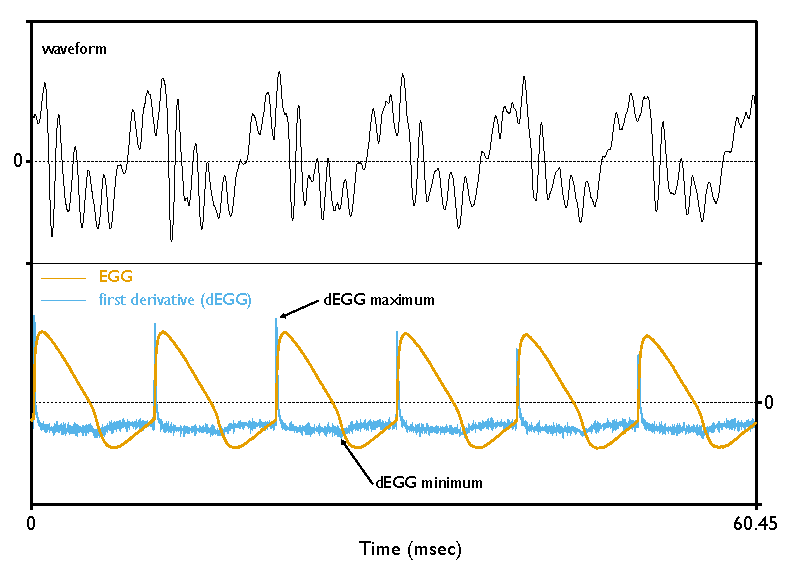
\includegraphics{./img/degg-signal.pdf}
  \caption{The electroglottographic signal (EGG) with corresponding first derivative (dEGG).}
  \label{f:egg}
\end{figure}

An example EGG signal is provided in \Cref{f:egg}. A glottal cycle can
be described in terms of two phases \citep{childers1985, hampala2016}:
(a) a contacting phase, in which the vocal folds are approaching each
other, (c) a de-contacting phase, in which the vocal folds move apart
from each other. Transversal to this two-phase description, the glottal
cycle can be described in terms of whether the glottis is occluded or
not. So the cycle can be divided into (1) a closed phase, in which the
glottis is completely closed and glottal flow is 0 (in some contexts
this phase could be absent, like in breathy voicing), and (2) an open
phase, in which there is no complete occlusive contact between the vocal
folds. The timing of these phases can be approximated from the EGG
signal, as demonstrated by both experimental and modelling work.

Two important landmarks of glottal movement are the closing instant (the
timepoint of glottal complete closure) and the opening instant (the
moment in which the glottis first opens). These points delimit the open
and closed phases of a glottal cycle. The ratio of the closed phase
relative to the total cycle duration, the closed quotient, has been used
as an index of phonation mode. Modal voice has higher CQ values than
breathy voice, and lower values than creaky voice. One method for the
detection of the closing and opening instants is based on the first
derivative of the EGG signal (dEGG, see \Cref{f:egg}).
\citet{herbst2017} showed that this method returns values that are just
a surrogate of the actual articulatory closing and opening instants, due
to the complex anatomy of the vocal folds, and recommends to call this
EGG-based closed quotient the `contact quotient'.

As an alternative to contact quotient, \citet{herbst2010} propose a
visualisation method, the wavegram, which does not reduce the EGG signal
to a single value, but rather uses information from the whole signal to
qualitatively assess vocal folds activity. A wavegram is a 3D
representation of the EGG signal developing in time. Its structure is
similar to that of a classical phonetic spectrogram. On the
\emph{x}-axis, the indexes of individual glottal cycles are laid out
sequentially. The \emph{y}-axis is the time within each glottal cycle,
normalised between 0 and 1. Finally, the amplitude of the signal
normalised between 0 and 1 within each glottal cycle (the third
dimension) is represented by different colour intensities. Differences
in intensity along the \emph{x}-axis indicate changes in glottal
activity. The procedure for constructing a wavegram is given in
\Cref{f:wavegram}. A wavegram can be produced for the EGG signal and for
any transformation, like the dEGG.

\begin{figure}
  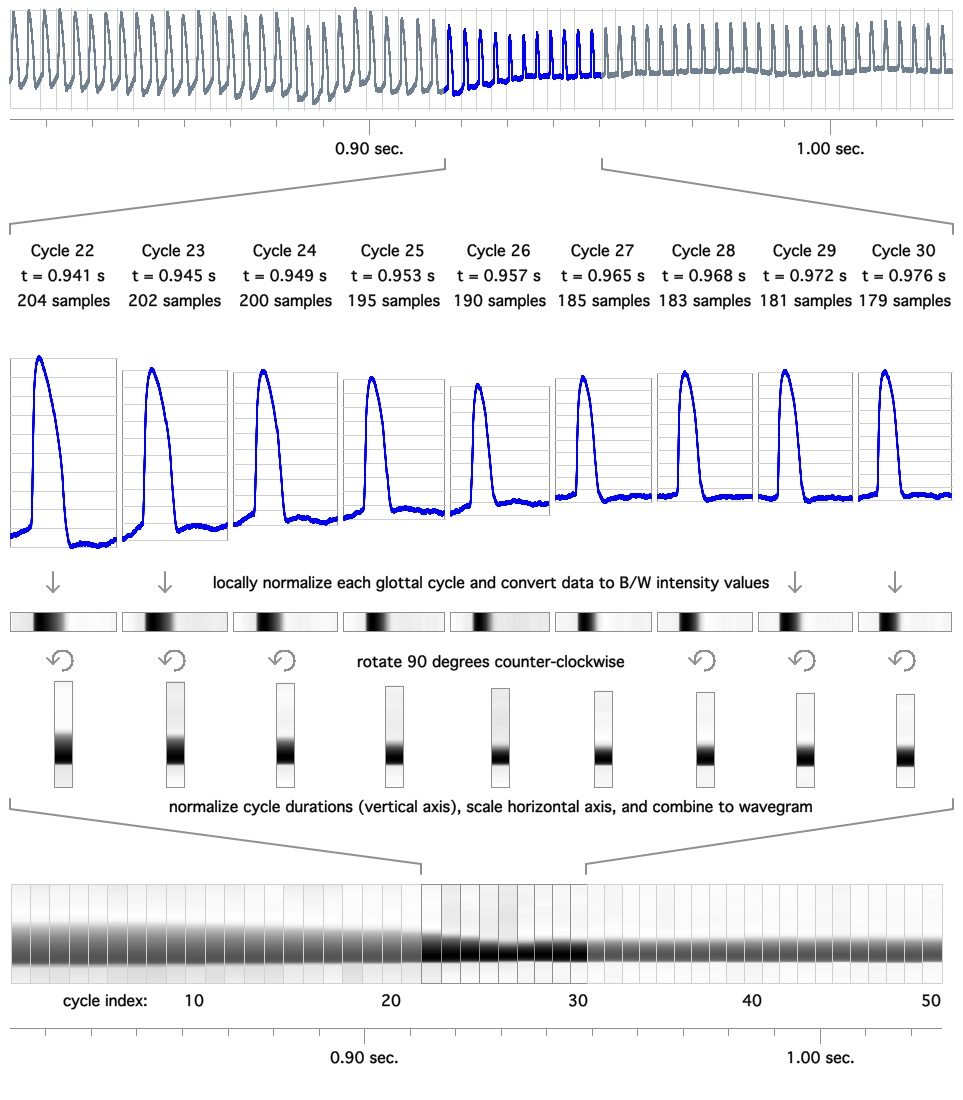
\includegraphics{./img/wavegram.png}
  \caption{The wavegram. Created by Christian T. Herbst under a CC BY-SA 3.0 license.}
  \label{f:wavegram}
\end{figure}

A possible limitation of the wavegram method is that it is intended for
a qualitative analysis based on visual inspection. However, wavegram
data can be modelled using generalised additive models (GAMs,
\citealt{hastie1986, zuur2012, wood2017}). GAMs are a family of
generalised models which can fit non-linear effects by additive
combinations of smoothing splines. The flexibility of GAMs allows
researchers to generate a fitted wavegram based on data from multiple
repetitions of a single speaker and from multiple speakers. Random
effects can also be included to account for idiosyncratic differences.
Moreover, the potential of overfitting due to the flexibility of GAMs is
reduced by a smoothing penalty parameter, which constraints the maximum
number of basis functions used to construct the smoothing splines. This
paper introduces wavegram GAMs as a way to quantitatively assess
wavegram data. First, the results from a pilot study which informally
evaluates the proposed method are presented (\Cref{s:pilot}).
\Cref{s:voicing} illustrates how to conduct a wavegram GAM analysis of
dEGG wavegram data through a practical example which compares the
wavegrams of vowels followed by voiceless and voiced stops. Finally,
\Cref{s:limits} discusses limitations of the current implementation of
the method and future directions.

\hypertarget{pilot-study}{%
\section{Pilot study}\label{pilot-study}}

\label{s:pilot}

Synchronised audio and electroglottographic (EGG) data were obtained
from 5 trained phoneticians, who were asked to produce sustained tokens
of /a/ with modal and breathy voice. The data was collected using a
Glottal Enterprises EG2-PCX2 electroglottograph and a Movo LV4-O2
Lavalier microphone, at a sample rate of 44100 Hz (16-bit). The
acquisition of the signals was controlled with Audacity running on a
MacBook Pro (Retina, 13-inch, Mid 2014). The placement of the electrodes
strap was checked with the height indicator on the EGG unit. Each
participant uttered 10 consecutive tokens of a sustained /a/ in modal
voice, followed by 10 tokens of a sustained breathy /a/. All subsequent
data processing was performed in Praat \citep{boersma2018}. The onset
and offset of each token were detected with an automatic procedure which
finds voiced and unvoiced intervals (\texttt{To\ TextGrid\ (vuv)}). The
dEGG wavegram data was extracted from the first 8 glottal cycles of a
500 ms window centred around the mid-point of each token. From each
glottal cycle, the relative amplitude of the dEGG signal was extracted
every 10 samples.

A generalised additive mixed model (GAMM) was fitted to the data to
statistically assess differences in vocal fold activity between modal
and breathy voicing. The following terms were included: the amplitude of
the dEGG signal as the outcome variable, a factor with language and
phonation as a parametric term, a smooth over the normalised time of the
beginning of the glottal cycle (as the proportion of the time relative
to the entire token duration) and one over the normalised time of the
sample within the glottal cycle (as the proportion of the time relative
to the duration of the glottal cycle), two difference smooth over
normalised time of the glottal cycle onset and normalised sample time
using a by-variable with the language/phonation factor, a tensor product
interaction between normalised cycle time and normalised sample time and
the same tensor product interaction with a language/phonation
by-variable. Finally, by-speaker differences were modelled with a
by-speaker factor smooth over normalised cycle time. A first-order
autoregressive (AR1) model was included to deal with the relatively high
auto-correlation in the residuals.

\Cref{f:surface-p} shows the modelled wavegrams of the modal and breathy
tokens. Since the tokens were produced with sustained phonation, no
appreciable change within each wavegram can be observed. However, the
comparison of the wavegram of modal voice with that of breathy voice
reveals clear differences. As a general trend, the dEGG maximum is
achieved later within the glottal cycle in breathy voicing relative to
modal voicing. This is compatible with the lower CQ values observed in
breathy voicing. Moreover, differences in velocity of closing and
opening movements of the folds are signalled by the relative widths of
the red-coloured (around the dEGG maximum) and the blue-coloured bands
(around the dEGG minimum). While in modal voicing the blue band is
wider, the red band is in breathy voice, indicating that the velocity
into and out of the beginning of the closed phase is slower in breathy
voicing.

\begin{figure}
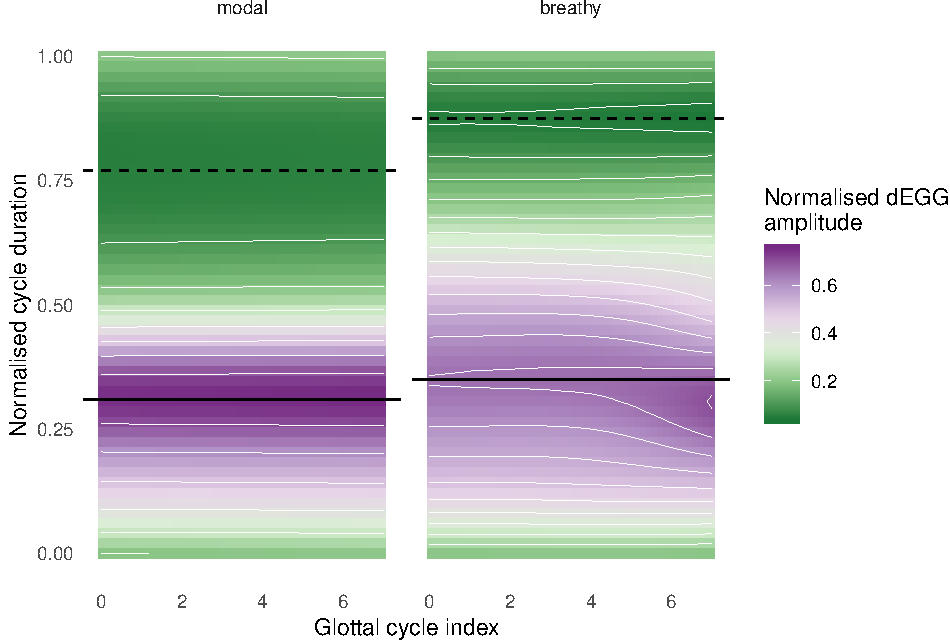
\includegraphics[width=\linewidth]{2019-wavegram_files/figure-latex/surface-p-1} \caption{Fitted wavegram of modal and breathy phonation (\Cref{s:pilot}).}\label{f:surface-p}
\end{figure}

\hypertarget{wavegram-of-vowels-followed-by-voiceless-vs.-voiced-stops}{%
\section{Wavegram of vowels followed by voiceless vs.~voiced
stops}\label{wavegram-of-vowels-followed-by-voiceless-vs.-voiced-stops}}

\label{s:voicing}

This section further illustrates the use of wavegram GAMs by discussing
a dynamic analysis of changes in vocal folds activity during the
production of vowels followed by voiceless vs.~voiced stops in Italian
and Polish. EGG data was obtained from 9 Italian speakers and 6 Polish
speakers. The procedures for data processing and analysis were the same
as with the pilot study, with the exception that data was extracted from
every glottal cycle within the whole duration of the vowel. The vowel
onset and offset were identified as the appearance and disappearance of
higher formant structure respectively \citep{machac2009}.

\begin{figure}
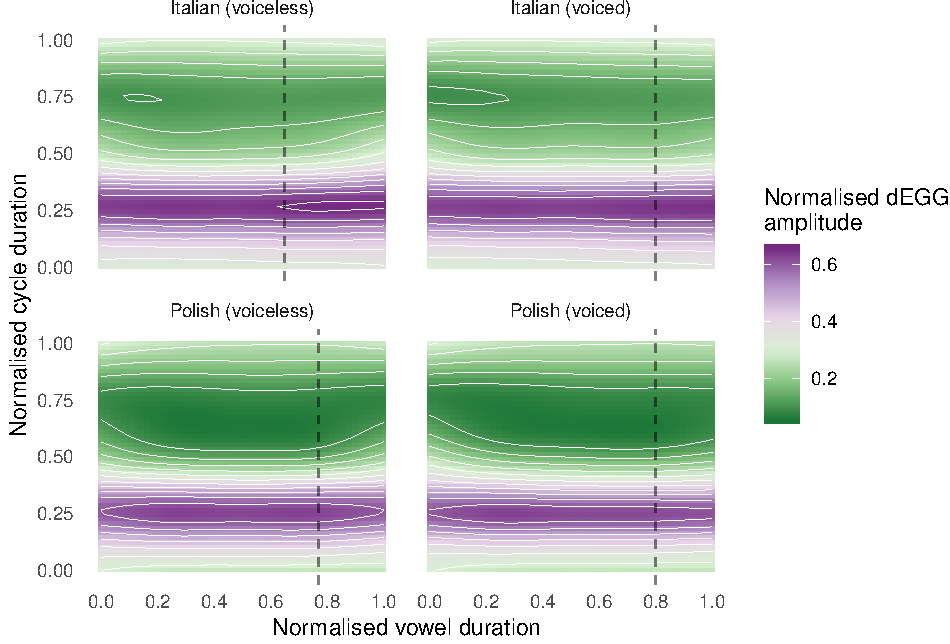
\includegraphics[width=\linewidth]{2019-wavegram_files/figure-latex/surface-1} \caption{Fitted wavegram of vowels followed by voiceless and voiced stops in Italian and Polish (\Cref{s:voicing}).}\label{f:surface}
\end{figure}

\Cref{f:surface} shows the modelled wavegrams of vowels followed by
voiceless (left) and voiced stops (right), in Italian (top) and Polish
(bottom). The wavegrams indicate that vocal folds activity changes
towards the end of the vowel if the following consonant is voiceless,
both in Italian and Polish. The glottal activity along the second half
of vowels followed by voiced stops is, on the other hand, more stable.
Moreover, the change in activity is initiated earlier in Italian (at
around 60\% into the vowel) than in Polish (at about 80\%). What the
wavegrams show is that glottal opening increases towards the end of the
vowel, in anticipation of the open glottis typical of voiceless stops
(and consonants more in general).

Another difference between the two languages concerns the initial
voiceless stop (/p/). The change observed between 50 and 70\% into the
glottal cycle at the beginning of the vowel, which indicates a
transition from a more spread glottis, is more extreme in Polish than in
Italian. This means that phonation at vowel onset is slightly breathier
in the former. Such difference is compatible with the finding that
Polish voiceless stops have on average a longer VOT than Italian stops.

The observation of increased glottal opening in the production of vowels
followed by voiceless stops in Italian is further compatible with the
reported presence of pre-aspiration (breathy or voiceless) in Italian
geminate stops
\citep{stevens2004, stevens2004a, stevens2010, stevens2010b, stevens2014a}.
Increased glottal spreading during vocal fold vibration is the logical
precursor of voiceless pre-aspiration. The fact that voiceless
pre-aspiration is not fully developed in Italian singleton voiceless
stops offers interesting insights concerning the duration of voiceless
stops and the emergence of pre-aspiration.

It is known that voiceless stops have longer closure durations than
voiced stops. \citet{lisker1974} argues that, in English voiceless
stops, closure occurs not long after the spreading gesture is initiated
in order to avoid the emergence of full pre-aspiration. There are,
however, varieties of English with pre-aspiration in stops and
fricatives \citep{gordeeva2007, nance2013, hejna2015a}. The question
arises as to how glottal spreading in vowels in the context of voiceless
stops can lead to the emergence of pre-aspiration in some cases. One of
the common conceptions is that pre-aspiration arises when closure
duration decreases while glottal spread remains. \citet{nichasaide1985},
however, claims that the appearance of pre-aspiration (in the form of
glottal spread before stop closure) diachronically precedes closure
shortening. \citet{stevens2014} further present experimental evidence
from Italian that pre-aspiration and closure shorting are independent.
Moreover, the presence of pre-aspiration increased the total duration of
the VC sequence.

What can be learnt from this is that, once breathyness/pre-aspiration
arises, there are two possible scenarios: according to one possible
path, as noted by \citet{lisker1974}, pre-aspiration is prevented by
achieving stop closure earlier (thus increasing the stop closure
duration); according to the other path, pre-aspiration can be enhanced,
with subsequent closure shortening, as in the arguments by
\citet{nichasaide1985} and \citet{stevens2014}.

\bibliography{linguistics}


\end{document}
